%& -job-name=newfilenameialwayswanted

\documentclass[12]{beamer}

\usepackage[T1]{fontenc}
\usepackage[utf8]{inputenc}
\usepackage[polish]{babel}

\usetheme{Warsaw}
\usecolortheme{seahorse}%{lily} 
%\setbeamercolor{frametitle}{bg=yellow,fg=blue} 
%\beamersetaveragebackground{blue!10} 

\colorlet{mystruct}{structure} % Zapis struktury
\colorlet{structure}{magenta} % Nowa struktura
\definecolor{kolor1}{RGB}{255,255,255}
\definecolor{kolor2}{RGB}{132,5,5}
\setbeamercolor{structure}{fg=kolor2} %kolor struktury (wypunktowania, spis tresci itp)
\setbeamercolor{palette primary}{fg=kolor2,bg=kolor1} %kolor ”tego” z podrozdzialami i \frametitle{}
\setbeamercolor{palette quaternary}{fg=kolor1,bg=kolor2} %kolor ”tego” z rozdzialami
\setbeamercolor{normal text}{fg=black,bg=kolor1}
%normalny tekst i tlo
\setbeamercolor{titlelike}{parent=palette quaternary}
%kolory tytulu jak w palete quaternary
\setbeamercolor{block title}{fg=kolor1,bg=kolor2}
%tytul bloku, napis i tlo
\setbeamercolor{block body}{parent=palette primary,fg=black} %kolor ciala bloku

\usepackage[T1]{fontenc}
\usepackage[utf8]{inputenc}
\usepackage[polish]{babel}

\usepackage{graphicx}
%\usepackage{array}
%\usepackage{amssymb}


\title[Zastosowanie sztucznej inteligencji w wykrywaniu niechcianej poczty elektronicznej]
{Zastosowanie sztucznej inteligencji w wykrywaniu niechcianej poczty elektronicznej}

\author{Paweł Siwoń} % \\ Supervisor's name and surname}
\institute[ICS, TUL]{dr hab. inż. Tomasz Hyla, - prof. ZUT} % Institute of Information Technology, Lodz University of Technology, Poland}
\date{Styczeń 2025}

%\AtBeginSubsection[]
%{
%  \begin{frame}<beamer>{Outline}
%    \tableofcontents[currentsection,currentsubsection]
%  \end{frame}
%}

\begin{document}

\begin{frame}
  \titlepage
\end{frame}

\begin{frame}{Outline}
  \tableofcontents
  % You might wish to add the option [pausesections]
\end{frame}

\section{Wstęp}

\subsection{Motywacja}

\begin{frame}{Dziedzina pracy magisterskiej}
\normalsize{
  \begin{itemize}
  \item
    \textbf{Opis aktualnej sytuacji w wybranej dziedzinie IT:}
    \begin{itemize}
        \item Wykorzystanie poczty elektronicznej jako podstawowego narzędzia komunikacji w biznesie i życiu codziennym.
        \item Rosnąca liczba zagrożeń związanych z niechcianą pocztą elektroniczną (np. spam, phishing), stanowiąca poważne ryzyko dla użytkowników oraz organizacji.
        \item Wykorzystanie sztucznej inteligencji (AI) w cyberbezpieczeństwie, w tym w rozwoju metod wykrywania niechcianej poczty.
    \end{itemize}
  \end{itemize}
}
\end{frame}

\begin{frame}{Cel i zakres pracy magisterskiej}
\normalsize{
  \begin{itemize}
  \item
    \textbf{Cel} pracy magisterskiej
  \begin{itemize}
    \small{
    \item
      Analiza i rozwój metod klasyfikacji poczty elektronicznej z wykorzystaniem sztucznej inteligencji w celu wykrywania różnych kategorii niechcianych wiadomości, takich jak spam i phishing.
     \item
      Stworzenie efektywnego rozwiązania, które można wdrożyć w środowisku produkcyjnym, działającego na serwerze pocztowym lub lokalnie na urządzeniu klienta.
    }
  \end{itemize}
  \end{itemize}
}
\end{frame}

\begin{frame}{Cel i zakres pracy magisterskiej}

\normalsize{
  \begin{itemize}
  \item
    \textbf{Zakres} pracy magisterskiej
  \begin{itemize}
  \small{
    \item
      Wprowadzenie do tematyki cyberbezpieczeństwa związanego z pocztą elektroniczną i omówienie zagrożeń, takich jak spam i phishing.
    \item
      Analiza istniejących metod wykrywania niechcianej poczty, w tym technik opartych na sztucznej inteligencji.
    \item
      Przygotowanie zbiorów danych testowych złożonych z różnych typów wiadomości email.
    \item
      Testowanie i porównanie co najmniej trzech technik AI pod kątem skuteczności wykrywania niechcianych wiadomości.
    \item
      Implementacja prototypu aplikacji do wykrywania niechcianej poczty, uwzględniającej możliwość integracji z serwerem pocztowym.
    \item
      Wnioski oraz propozycje dalszego rozwoju aplikacji.
    }
  \end{itemize}
  \end{itemize}
}
\end{frame}

  

\subsection{Istniejace rozwiązania problemu}

\begin{frame}{Istniejące rozwiązania problemu}
\normalsize{
  \begin{itemize}
  \setbeamercovered{transparent}
  \item
    Istniejące rozwiązania praktyczne -- aplikacje / systemy informatyczne
    \begin{itemize}
    \small{
    \item
      Filtry bazujące na regułach (np. SpamAssassin) -- wykorzystanie zdefiniowanych reguł do klasyfikacji wiadomości.
    \item
      Systemy oparte na statystycznych modelach klasyfikacji (np. Bayesowskie filtry spamu).
    \item
      Rozwiązania bazujące na uczeniu maszynowym, takie jak algorytmy wspierające w Gmail czy Outlook.
   
    }
  \end{itemize}
  \end{itemize}
}
\end{frame}

\begin{frame}{Istniejące rozwiązania praktyczne}
\normalsize{
  \begin{itemize}
  \setbeamercovered{transparent}
  \item
    Analiza istniejących rozwiązań -- zalety i wady
    \begin{itemize}
    \small{\item
      Filtry regułowe: proste w implementacji, ale podatne na obejście przez dynamicznie zmieniające się techniki 
    \item
      Modele statystyczne: skuteczne w podstawowych przypadkach, lecz wymagające regularnego trenowania i dostosowania.
    \item
      Rozwiązania oparte na uczeniu maszynowym: wysokie wskaźniki skuteczności, ale często obarczone dużymi wymaganiami obliczeniowymi oraz podatnością na brak dostępu do odpowiednich zbiorów danych.
    }
  \end{itemize}
  \end{itemize}
}
\end{frame}

\begin{frame}{Istniejące rozwiązania praktyczne}
\normalsize{
  \begin{itemize}
  \setbeamercovered{transparent}
  \item
    Wyniki analizy -- potrzeba nowego rozwiązania opartego o duże modele językowe
    \begin{itemize}
    \small{
    \item
      Istnieje potrzeba stworzenia systemu, który łączy efektywność metod AI z możliwością działania w środowisku rzeczywistym.
    \item
      Konieczne jest opracowanie rozwiązania odpornego na zmieniające się techniki ataków, które będzie wydajne i łatwe do integracji z istniejącymi systemami.
    \item
      Wskazane jest uwzględnienie aspektów takich jak ochrona prywatności i minimalizacja fałszywie pozytywnych klasyfikacji.
    }
  \end{itemize}
  \end{itemize}
}
\end{frame}


\section{Rozwiązanie problemu}

\subsection{Jak rozwiązać problem?}

\begin{frame}{Plan pracy magisterskiej}
\normalsize{
  \begin{itemize}
  \item
    Wstępny plan pracy magisterskiej
  \begin{enumerate}
    \small{
    \item
      Wprowadzenie teoretyczne:
      \begin{itemize}
      \item Analiza zagrożeń związanych z niechcianą pocztą elektroniczną (spam, phishing).
      \item Przegląd istniejących metod wykrywania niechcianych wiadomości, w tym rozwiązań opartych na sztucznej inteligencji.
      \end{itemize}
    \item
      Przygotowanie środowiska badawczego:
      \begin{itemize}
      \item Zebranie zbiorów danych testowych zawierających różne typy wiadomości email.
      \item Wstępna analiza i preprocessing danych.
      \end{itemize}
    \item
      Eksperymentalna analiza metod sztucznej inteligencji:
      \begin{itemize}
      \item Wybór trzech różnych algorytmów AI (np. BERT, RoBERT, GPT, Gemini, OLLAMA).
      \item Przeprowadzenie testów skuteczności metod na przygotowanych zbiorach danych.
      \end{itemize}
    }
  \end{enumerate}
  \end{itemize}
}
\end{frame}

\begin{frame}{Plan pracy magisterskiej}
\normalsize{
  \begin{itemize}
  \item
    Wstępny plan pracy magisterskiej
  \begin{enumerate}
  	\setcounter{enumi}{3}
    \small{
    \item
      Implementacja prototypu aplikacji:
      \begin{itemize}
      \item Opracowanie aplikacji działającej na serwerze pocztowym lub lokalnie.
      \item Integracja z istniejącymi systemami pocztowymi.
      \end{itemize}
    \item
      Ewaluacja wyników:
      \begin{itemize}
      \item Analiza skuteczności aplikacji w wykrywaniu niechcianych wiadomości.
      \item Omówienie zalet i ograniczeń zastosowanego podejścia.
      \end{itemize}
    \item
      Wnioski i propozycje dalszego rozwoju:
      \begin{itemize}
      \item Podsumowanie wyników pracy.
      \item Możliwości rozszerzenia aplikacji o dodatkowe ulepszenia.
      \end{itemize}
    }
  \end{enumerate}
  \end{itemize}
}
\end{frame}


\subsection{Jak rozwiązać problem poprzez implementację?}

\begin{frame}{Plan implementacji pracy magisterskiej}
\normalsize{
  \begin{itemize}
  \setbeamercovered{transparent}
  \item
    wstępny plan implementacji pracy magisterskiej (część praktyczna pracy magisterskiej)
    \begin{enumerate}
    \small{
    \item
      Projekt oraz implementacja aplikacji integrującej LLM z usługą SMTP
    \item
      Przygotowanie / pozyskanie zbiorów danych weryfikujących
    \item
      Przeprowadzenie eksperymentów
    \item
      Analiza wyników
    }
  \end{enumerate}
  \end{itemize}
}
\end{frame}


\begin{frame}{Przykładowy rysunek}
  \begin{figure}[t]
    \centering
    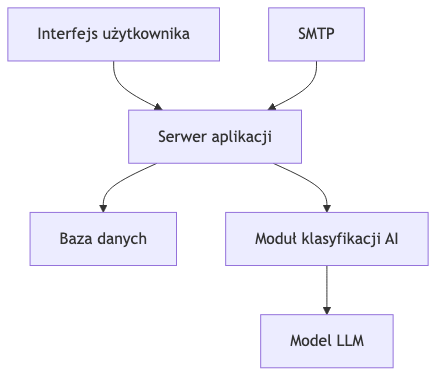
\includegraphics[height=4cm]{images/app_arch.png}
  \end{figure}
\end{frame}


\begin{frame}{Przykładowy rysunek}
  \begin{figure}[t]
    \centering
    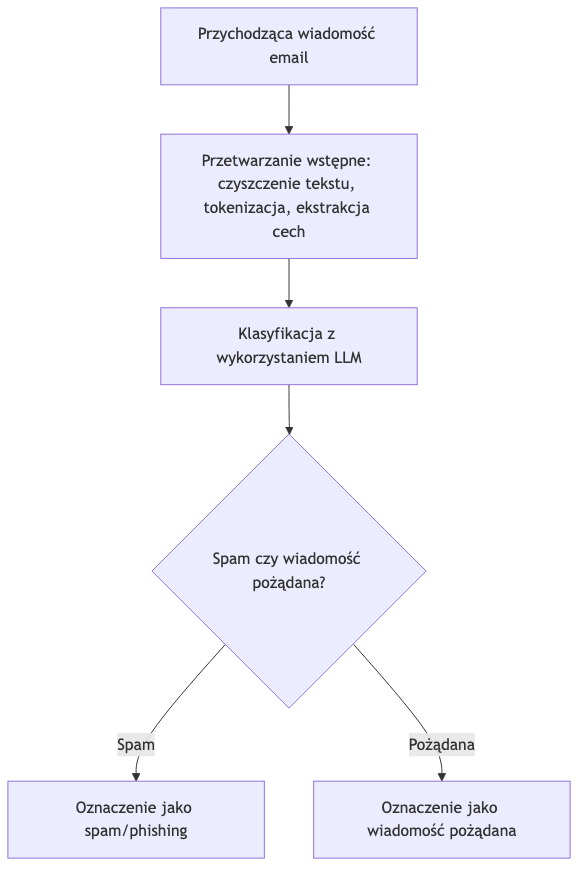
\includegraphics[height=6cm]{images/diagram.png}
  \end{figure}
\end{frame}

\section{Podsumowanie}

\begin{frame}{Podsumowanie}
\normalsize{
  \begin{itemize}
  \item
    ...
  \item
    ...
  \end{itemize}
}
\end{frame}

\begin{frame}{Conclusions}
	\center
		{Dziękuję za uwagę}
\end{frame}

\end{document}

